%% template_demo.tex -- exercises every element of cs259.cls at realistic
%% density (title block, abstract, three heading levels, equations, figures,
%% tables, listing, citations, balanced last page).  The text is filler
%% about a made-up benchmark; none of the numbers are results of the study.
%%
%% Build:  python3 make_demo_figs.py         (creates demo_figs/*.pdf)
%%         pdflatex template_demo ; bibtex template_demo ;
%%         pdflatex template_demo ; pdflatex template_demo
%%    or   tectonic template_demo.tex
\documentclass[siunitx]{cs259}

\hypersetup{pdftitle={CS 259 template demo},
            pdfauthor={Sunnihith Reddy Induru}}

%% Demo bibliography written at compile time, so this file is self-contained.
\begin{filecontents*}[overwrite]{demo_refs.bib}
@article{lecun98,
  author  = {Yann LeCun and L{\'e}on Bottou and Yoshua Bengio and Patrick Haffner},
  title   = {Gradient-based learning applied to document recognition},
  journal = {Proceedings of the IEEE},
  volume  = {86}, number = {11}, pages = {2278--2324}, year = {1998}}
@inproceedings{krizhevsky12,
  author    = {Alex Krizhevsky and Ilya Sutskever and Geoffrey E. Hinton},
  title     = {ImageNet classification with deep convolutional neural networks},
  booktitle = {Advances in Neural Information Processing Systems 25},
  pages     = {1097--1105}, year = {2012}}
@book{kirk16,
  author    = {David B. Kirk and Wen-mei W. Hwu},
  title     = {Programming Massively Parallel Processors: A Hands-on Approach},
  publisher = {Morgan Kaufmann}, edition = {3rd}, year = {2016}}
@book{chapman08,
  author    = {Barbara Chapman and Gabriele Jost and Ruud van der Pas},
  title     = {Using {OpenMP}: Portable Shared Memory Parallel Programming},
  publisher = {MIT Press}, year = {2008}}
@misc{openmp52,
  author       = {{OpenMP Architecture Review Board}},
  title        = {{OpenMP} Application Programming Interface, Version 5.2},
  year         = {2021},
  url          = {https://www.openmp.org/specifications/}}
@misc{cudaguide,
  author = {{NVIDIA Corporation}},
  title  = {{CUDA} {C++} Programming Guide},
  year   = {2024},
  url    = {https://docs.nvidia.com/cuda/cuda-c-programming-guide/}}
@inproceedings{amdahl67,
  author    = {Gene M. Amdahl},
  title     = {Validity of the single processor approach to achieving large
               scale computing capabilities},
  booktitle = {Proceedings of the AFIPS Spring Joint Computer Conference},
  pages     = {483--485}, year = {1967}}
@inproceedings{abadi16,
  author    = {Mart{\'\i}n Abadi and Paul Barham and Jianmin Chen and others},
  title     = {{TensorFlow}: A system for large-scale machine learning},
  booktitle = {Proceedings of the 12th USENIX Symposium on Operating Systems
               Design and Implementation (OSDI)},
  pages     = {265--283}, year = {2016}}
\end{filecontents*}

\title{Performance Evaluation of Hybrid CPU-GPU Parallelism\\
       for Deep Learning Using OpenMP and CUDA}
\author{Sunnihith Reddy Induru}
\affiliation{Computer Science Department\\
             San Jose State University\\
             San Jose, CA 95192}
\email{sunnihithreddy.induru@sjsu.edu}

\begin{document}
\maketitle

\begin{abstract}
This demonstration paper exercises every typographic element of the CS~259
term-paper class: the title block, an unnumbered abstract, numbered section,
subsection and subsubsection heads, justified Times body text, inline and
display equations, one-column and two-column figures with captions below,
one-column and two-column tables with captions above, a code listing, and a
numbered reference list sorted alphabetically by first author. The text is
placeholder material about a made-up benchmark; none of its numbers are
results of the study.
\end{abstract}

\section{Introduction}
Training deep neural networks is dominated by dense linear algebra that maps
naturally onto data-parallel hardware \cite{lecun98,krizhevsky12}. A modern
workstation offers two such engines: a multicore CPU programmed with OpenMP
\cite{openmp52,chapman08} and a GPU programmed with CUDA
\cite{cudaguide,kirk16}. This paper compares four implementations of the same
workload: a serial baseline, an OpenMP version, a CUDA version, and a hybrid
version that divides each mini-batch between the two devices.

The contributions of this demonstration are purely typographic. They are
listed here to give the introduction a realistic density:
\begin{itemize}
  \item a serial baseline whose output defines correctness;
  \item an OpenMP version that parallelises the batch loop
    (\code{\#pragma omp parallel for});
  \item a CUDA version using one thread per output element; and
  \item a hybrid version that splits each batch between CPU and GPU.
\end{itemize}
Section~\ref{sec:impl} describes the implementations,
Section~\ref{sec:method} the methodology, and Section~\ref{sec:results}
the results shown in Figure~\ref{fig:speedup}, Figure~\ref{fig:wide}, and
Tables~\ref{tab:cfg} and~\ref{tab:res}.

\section{Background and Related Work}
Amdahl observed that the serial fraction of a program bounds the achievable
speedup \cite{amdahl67}. If a fraction $f$ of the work is parallelisable over
$p$ processing elements, the speedup is
\begin{equation}
  S(p) \;=\; \frac{T_1}{T_p} \;=\; \frac{1}{(1-f) + f/p},
  \label{eq:amdahl}
\end{equation}
so that $S(p)\to 1/(1-f)$ as $p\to\infty$. For a hybrid CPU-GPU run the
effective throughput is the sum of the device throughputs,
$\Theta=\Theta_{\mathrm{cpu}}+\Theta_{\mathrm{gpu}}$, minus the cost of moving
data over the PCIe bus. Frameworks such as TensorFlow \cite{abadi16} hide
this placement from the user, which is convenient but makes controlled
comparisons difficult.

\subsection{Programming Models}
OpenMP expresses parallelism with compiler directives and a fork-join model,
whereas CUDA exposes an explicit grid of thread blocks. Both are described in
the standard references \cite{chapman08,kirk16}; we avoid repeating them and
instead concentrate on the practical differences that matter for the
experiments.

\subsubsection{Memory Hierarchy}
A CUDA kernel sees global, shared and register memory with a latency
difference of roughly two orders of magnitude, while an OpenMP thread sees a
conventional cache hierarchy. The distinction explains most of the
performance gap between the two versions in Section~\ref{sec:results}.

\subsubsection{Synchronisation}
OpenMP offers barriers and reductions; CUDA offers \code{__syncthreads()}
within a block and kernel boundaries across blocks.

\section{Workload and Dataset}
The workload is a small convolutional network trained on
\num{60000} grayscale images of $28\times28$ pixels. Each epoch performs
\SI{1.2e9}{} floating-point operations in the forward pass and about twice
that in the backward pass. The batch size is varied from \num{32} to
\num{512}.

\begin{table}[t]
\caption{Experimental configuration (placeholder values).}
\label{tab:cfg}
\begin{tabular}{@{}ll@{}}
\toprule
Item & Value \\
\midrule
CPU & 16 cores, \SI{3.0}{\giga\hertz} \\
GPU & \SI{16}{\giga\byte}, \SI{900}{\giga\byte\per\second} \\
Compiler & \code{gcc -O3 -fopenmp} \\
CUDA & \code{nvcc -O3 -arch=sm_80} \\
\bottomrule
\end{tabular}
\end{table}

\section{Implementations}\label{sec:impl}
\subsection{Serial CPU}
The baseline is a straightforward C++ implementation with no vectorisation
pragmas. It is the reference for correctness and for speedup.

\subsection{OpenMP}
The batch loop is parallelised with a \code{parallel for} directive and a
static schedule, as in Figure~\ref{lst:omp}. The number of threads is set
with \code{omp_set_num_threads}.

\begin{figure}[t]
\begin{lstlisting}[language=C++]
#pragma omp parallel for schedule(static)
for (int b = 0; b < batch; ++b) {
  forward(&x[b * D], &y[b * K]);
}
\end{lstlisting}
\caption{The OpenMP batch loop; a code excerpt set in a figure float so
that it is numbered and captioned like any other figure.}
\label{lst:omp}
\end{figure}

\subsection{CUDA}
Each thread computes one output element. The launch configuration uses 256
threads per block; \code{cudaMemcpyAsync} overlaps transfers with compute
when pinned host memory is used.

\subsection{Hybrid OpenMP-CUDA}
Each mini-batch is split into a CPU part and a GPU part whose sizes are
proportional to the measured device throughputs. The CPU part runs under
OpenMP while the GPU part runs asynchronously in a CUDA stream; the two are
joined at the end of every iteration.

\begin{figure}[t]
  \centering
  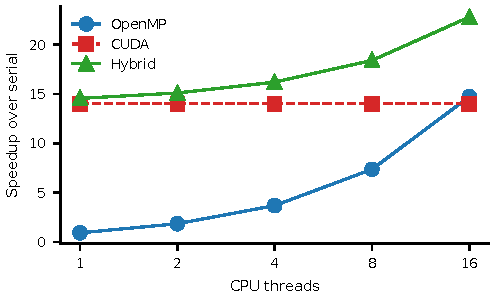
\includegraphics[width=\columnwidth]{demo_figs/demo_col.pdf}
  \caption{Speedup over the serial baseline versus CPU thread count
  (synthetic data). One-column figure, caption centered below.}
  \label{fig:speedup}
\end{figure}

\section{Experimental Methodology}\label{sec:method}
Every configuration is run ten times after two warm-up runs and the median is
reported. Wall-clock time is measured with \code{omp_get_wtime()} on the host
and with CUDA events on the device. The GPU is placed in a fixed performance
state, and the CPU governor is set to \code{performance} to reduce noise.

\subsection{Metrics}
We report time per epoch, speedup $S=T_{\mathrm{serial}}/T_{\mathrm{impl}}$,
and parallel efficiency $E=S/p$. For the GPU, $p$ is taken as one device.

\subsection{Reproducibility}
All code, build scripts and raw measurements are available at
\url{https://example.org/cs259/hybrid-dl}. Seeds are fixed so that the
serial and parallel versions produce identical initial weights.

\section{Correctness Validation}
The parallel versions are checked against the serial output after every
epoch. Floating-point reductions are not associative, so a relative tolerance
of $10^{-5}$ is used on the loss and $10^{-4}$ on the weights; all runs
satisfied both bounds.

\begin{figure*}[t]
  \centering
  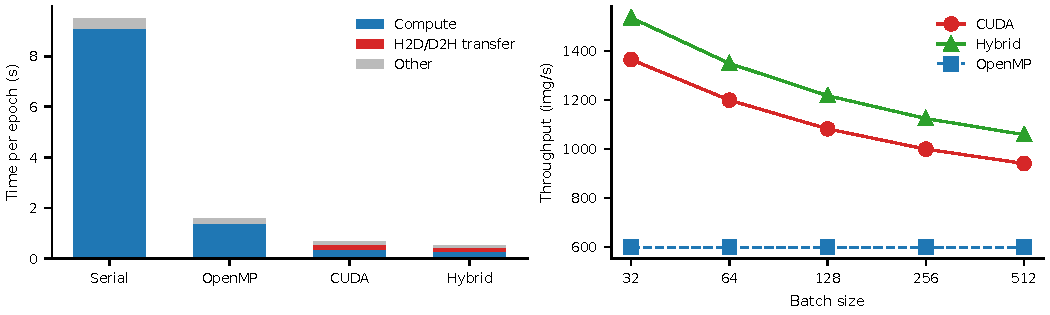
\includegraphics[width=\textwidth]{demo_figs/demo_wide.pdf}
  \caption{Time breakdown per epoch (left) and training throughput versus
  batch size (right), synthetic data. Two-column figure, caption centered
  below.}
  \label{fig:wide}
\end{figure*}

\section{Results}\label{sec:results}
Figure~\ref{fig:speedup} shows the OpenMP version scaling almost linearly up
to 16 threads, while the CUDA version is flat in the CPU thread count because
it does not use the CPU for compute. The hybrid version adds the CPU
contribution on top of the GPU, as predicted by the throughput model above.
Figure~\ref{fig:wide} breaks the epoch time into compute and transfer, and
shows that the transfer share shrinks as the batch size grows.

\begin{table*}[t]
\caption{Median time per epoch and speedup (synthetic data). Two-column table,
caption centered above.}
\label{tab:res}
\begin{tabular*}{\textwidth}{@{\extracolsep{\fill}}lrrrrrr@{}}
\toprule
 & \multicolumn{3}{c}{Batch size 64} & \multicolumn{3}{c}{Batch size 256} \\
\cmidrule(lr){2-4}\cmidrule(lr){5-7}
Implementation & Time (s) & Speedup & Eff. & Time (s) & Speedup & Eff. \\
\midrule
Serial CPU      & 9.50 & 1.0$\times$  & 1.00 & 9.12 & 1.0$\times$  & 1.00 \\
OpenMP (16 thr.)& 1.62 & 5.9$\times$  & 0.37 & 1.40 & 6.5$\times$  & 0.41 \\
CUDA            & 0.71 & 13.4$\times$ & ---  & 0.35 & 26.1$\times$ & ---  \\
Hybrid          & 0.58 & 16.4$\times$ & ---  & 0.30 & 30.4$\times$ & ---  \\
\bottomrule
\end{tabular*}
\end{table*}

\subsection{Scaling}
Parallel efficiency of the OpenMP version drops from $0.92$ at two threads to
$0.41$ at sixteen as memory bandwidth saturates. Equation~(\ref{eq:amdahl})
with $f=0.94$ predicts a limit of roughly $16\times$, which is consistent with
the measured $6.5\times$ at batch size 256 only if memory-bound phases are
counted as serial.

\subsection{Transfer Overhead}
At batch size 64 the host-device transfer takes about a quarter of the CUDA
epoch; at batch size 512 it falls below ten percent. Overlapping transfers
with compute in the hybrid version recovers most of that cost.

\section{Discussion}
The hybrid version is faster than either device alone in every configuration,
but the gain over CUDA is modest (about 18\% at batch size 64 and 14\% at
batch size 256) because the CPU contributes only a small fraction of the
total throughput. The balance point depends on the batch size, which suggests
adapting the split at run time rather than fixing it in advance.

\section{Limitations and Threats to Validity}
Results come from a single machine and a single network. Compiler versions,
driver versions and thermal state can change absolute numbers; relative
ordering was stable across repeated runs. The synthetic numbers in this
demonstration must not be quoted.

\section{Conclusion and Future Work}
We demonstrated the page layout of the CS~259 term-paper class. Future work
on the actual study includes a larger set of networks, power measurements and
a dynamic work-splitting policy.

\bibliographystyle{cs259}
\bibliography{demo_refs}

\end{document}
